\section{Transfert de données}
%\addcontentsline{toc}{section}{Transfert de données}
Le transfert de fichiers et de dossiers entre périphériques est possible depuis plusieurs sources et selon plusieurs protocoles. 
L'image qui suit montre une synchronisation à double sens en utilisant le logiciel sur P.C. --~flèches en rose~--, ou bien via le navigateur --~flèches en bleu~-- ou encore via l'application d'un smartphone ou d'une tablette --~flèches en rouge.
\begin{figure}
	\centering
	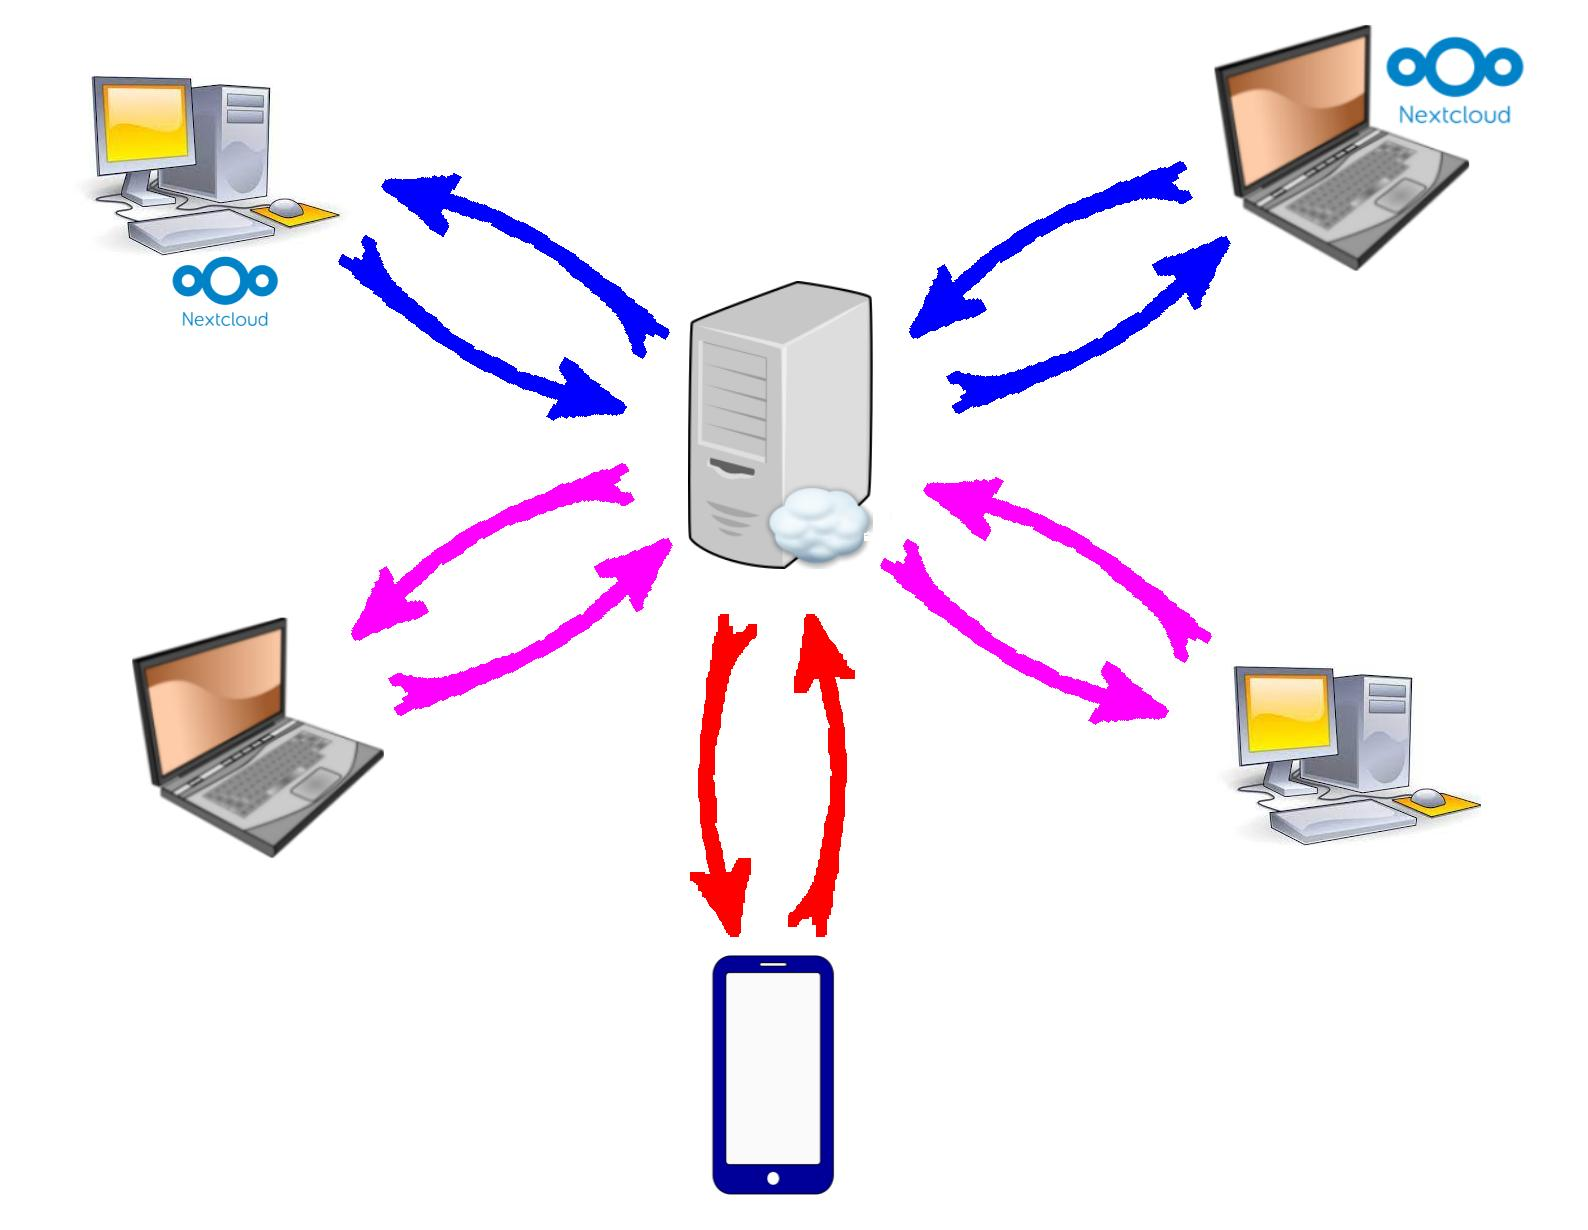
\includegraphics{./Captures/synchro.nextcloud.nuage.jpg}
	\caption{Le nuage est accessible par l'outil Nextcloud, par le navigateur, ou par le client smartphone pour transférer des données dans les deux sens.}
\end{figure}

\paragraph{La synchronisation via le client nextcloud pour ordinateur.} 
Comme le montre la capture d'écran du paragraphe \ref{fig-dossier-synchro}, transférer des fichiers entre l'ordinateur personnel et le nuage revient simplement à copier ou déplacer fichiers ou dossiers vers le dossier synchronisé, en soi on peut supposer que cette compétence est acquise par chaque lecteur.

Aussi dans les sous-sections suivantes ne seront abordés que le transfert de fichier par l'interface web.
De plus j'utiliserai le terme ``monter'' en lieu et place de l'anglicisme \emph{upload} et ``descendre'' parfois au lieu de télécharger.

\subsection{Monter un ou plusieurs fichiers}
%\addcontentsline{toc}{subsection}{Monter un ou plusieurs fichiers}
Tout se passe par l'icône en forme de rond avec une croix à l'intérieur, le {\Large $\oplus$} à gauche de la barre horizontale au dessus de l'espace réservé pour afficher les fichier. L'appui sur l'icône affiche le menu de la capture suivante~:
\begin{figure}
	\centering
	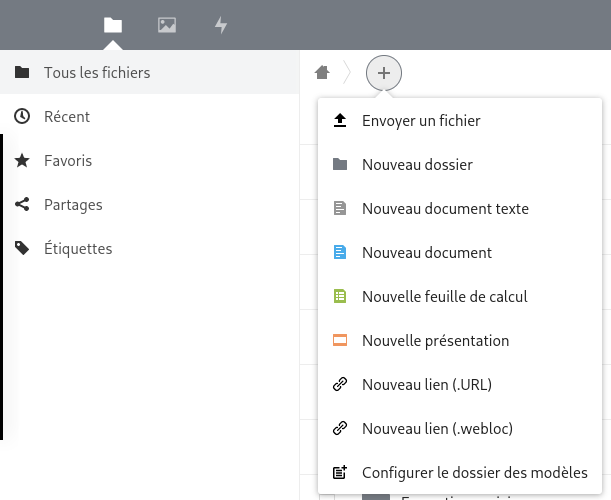
\includegraphics[width=0.5000\linewidth]{./Captures/nuage.menu.plus.png}
	\caption{Le menu ``plus''}
\end{figure}
En cliquant sur la ligne \og~Envoyer un fichier~\fg{} une fenêtre de l'explorateur local va s'ouvrir permettant de sélectionner un ou plusieurs fichiers qui seront envoyés dans le dossier affiché à l'écran.

\subsection{Créer un dossier}
%\addcontentsline{toc}{subsection}{Créer un dossier}
En cliquant sur la deuxième ligne du menu déroulant, c'est la création d'un dossier dans le dossier courant, attention il faut penser à clique sur la flèche au bout de la ligne pour valider le nom et créer le dossier.
\begin{figure}
	\centering
	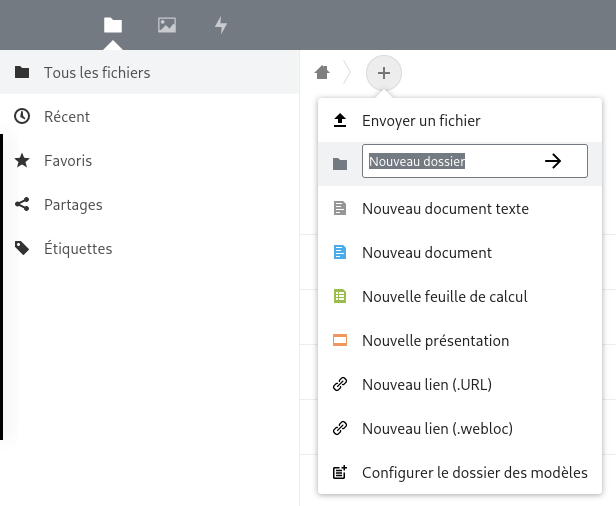
\includegraphics[width=0.5000\linewidth]{./Captures/nuage.menu.plus.creer.dossier.png}
	\caption{}
\end{figure}

Afin de valider la création d'un dossier, il suffit de saisir son nom et de valider par la touche entrée ou bien en cliquant sur la flèche en bout de ligne $\rightarrow$ et le dossier sera créé dans le dossier courant.

\subsection{Descendre un dossier ou plusieurs fichiers}
%\addcontentsline{toc}{subsection}{Descendre un dossier ou plusieurs fichiers}
L'un des avantages du nuage intégré à Apps.Education est la possibilité d'ouvrir, certes, mais aussi de télécharger ensuite un ou plusieurs fichiers, ou bien un ou plusieurs dossiers.

\begin{figure}
	\centering
	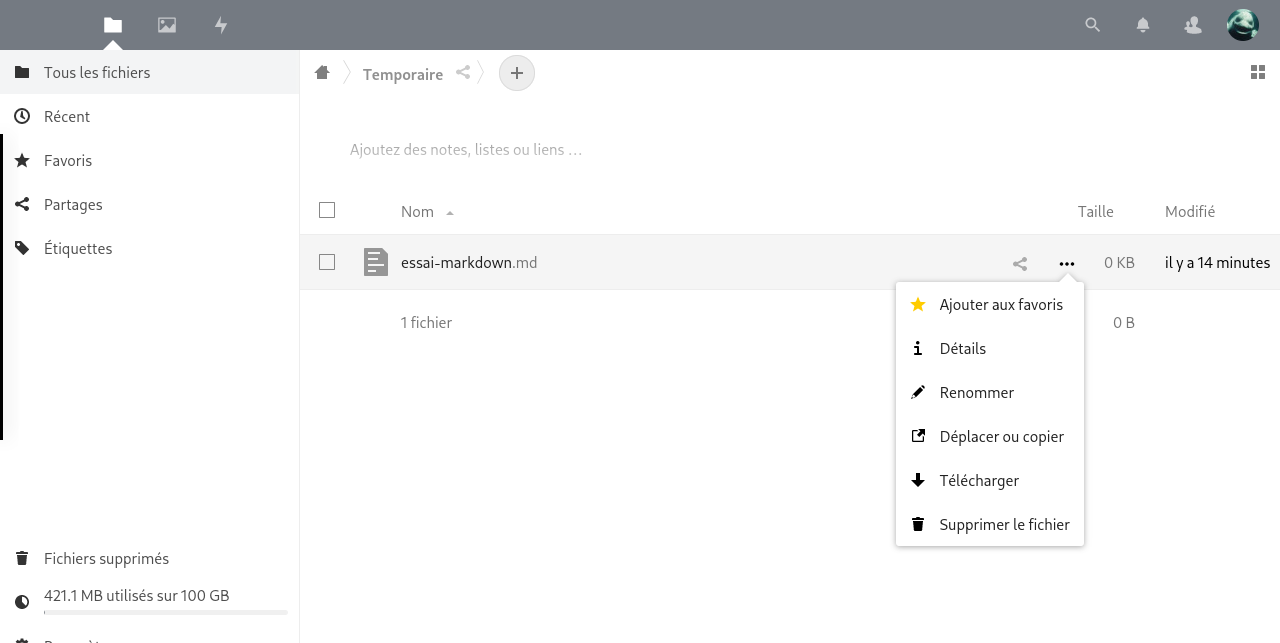
\includegraphics{./Captures/nuage.accueil.menu.contextuel.png}
	\caption{}
\end{figure}
Lorsqu'on appuie sur les \ldots un menu contextuel montre les différents choix proposés pour cet objet --~ici un fichier un texte balisé en langage \texttt{Markdown}. 

\subsection{Ce qui est spécifique au programme Nextcloud}
%\addcontentsline{toc}{subsection}{Ce qu'il n'est pas possible de faire} 
Par défaut, l'interface web du nuage ne permet pas d'envoyer directement un dossier, son contenu et toute la hiérarchie fille qui en découle, mais, cela reste possible par l'utilisation du client Nextcloud vu précédemment. 

Ouvrez deux fenêtres, l'une pointant le dossier synchronisé par le client Nextcloud, l'autre montrant la source des données à transférer, et, comme vous le feriez d'un dossier vers un dispositif externe, copiez ou déplacez les objets choisis (mélangeant tout ce que vous voulez de dossiers et de fichiers), quelques instants plus tard la synchronisation s'effectuera et créera dans le nuage les dossiers, les sous-dossiers et y placeront tous les fichiers quelque soit leur position dans l'arborescence.

Parmi les choix proposés, on peut renommer le fichier, le copier ou le déplacer --~c'est la même fenêtre mais pas le même bouton sur lequel cliquer~-- ou encore télécharger la ressource.

La règle est simple, si la ressource est un fichier simple, le fichier est téléchargé tel quel si par contre cela correspond à la sélection de plusieurs objets ou au moins d'un dossier, alors le nuage va compresser le tout dans une ressource unique, un fichier \emph{.zip} et c'est cet élément qui sera téléchargé.

\paragraph{Notez aussi.} 
On peut sélectionner un ou plusieurs objets en cliquant sur la case $\square$ en début de ligne, faisant apparaître en haut, à droite de \og~Nom~$\triangledown$~\fg{} comme le montre l'image qui suit.
\begin{figure}
	\centering
	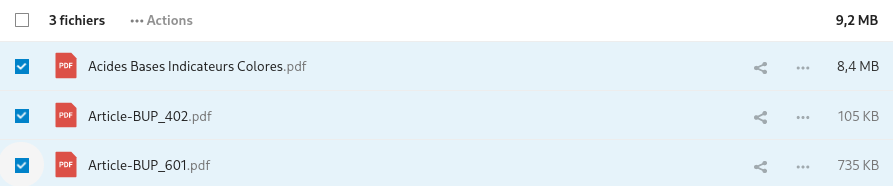
\includegraphics{./Captures/nuage.selection.plusieurs.objets.png}
	\caption{Sélection de plusieurs objets}
\end{figure}
on peut aussi sélection tous les objets du répertoire en cliquant sur le $\square$ tout en haut.
\begin{figure}
	\centering
	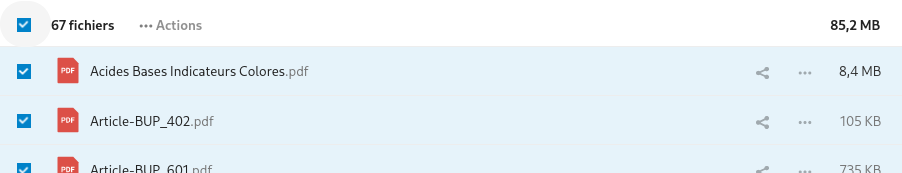
\includegraphics{./Captures/nuage.selection.tous.objets.png}
	\caption{Sélection complète}
\end{figure}